\section{Côté serveur}

	\subsection{Une API REST}
		Nous avons décider de proposer une API REST pour le serveur de notre application. Ce choix s'explique par la popularité de ce type d'API depuis plusieurs années, et surtout sa capacité à pouvoir être utilisée facilement (peu de firewalls bloquent le port 443 correspondant au HTTPS) et rapidement (tous les langages et frameworks proposent des méthodes d'accès à ce type d'API).

	\subsection{Nom de domaine et serveur}
		Nous avons réussi à récupérer gratuitement le domaine \texttt{diplo-lejeu.fr} grâce à une offre de Gandi (\url{https://www.gandi.net}). Nous avons acheté également un VPS Sandbox chez RunAbove (\url{https://www.runabove.com/instances/sandbox.xml}), filiale du groupe OVH, ayant 2 GB de RAM, 1 processeur et 20 GB de SSD.

	\subsection{Certificat HTTPS}
		Nous utilisons CloudFlare (\url{https://www.cloudflare.com}) pour gérer nos DNS et proposer un certificat HTTPS valide gratuitement, sur tous nos sous-domaines. Le trafic est chiffré entre le client et un des serveurs de CloudFlare en utilisant un certificat émis par Comodo, puis est chiffré à l'aide d'un certificat auto signé généré par nous-même entre CloudFlare et notre serveur RunAbove se trouvant à Roubaix en France.

	\subsection{Documentation de l'API REST}
		\subsubsection{Écriture en Markdown}
			La documentation de l'API REST est écrite en Markdown, langage de balisage léger et qui a été popularisé grâce aux forums et à GitHub. Les spécifications du langage ont toujours été floues, mais la syntaxe la plus commune actuellement est celle dite \textit{GitHub Flavored Markdown}\footnote{Une tentative de spécification précise du langage est actuellement proposée sous le nom de \enquote{CommonMark} à l'adresse \url{http://commonmark.org}.} (\url{https://help.github.com/articles/github-flavored-markdown/}), proposée par GitHub. Les fichiers composant la documentation de l'API sont disponibles sur GitHub à l'adresse \url{https://github.com/AntoineAugusti/diplo/tree/master/documentation-api}.\\

			Nous avons fait très attention à indiquer les différents endpoints disponibles, les paramètres à passer à l'endpoint, le détail de la réponse de l'API et toutes les erreurs possibles en respectant les règles de bonne pratique de conception et de sémantique d'API REST ainsi que le protocole HTTP.

		\subsubsection{Du Markdown au HTML}
			Nous utilisons un transformateur Markdown vers HTML pour proposer une interface web à notre API à l'aide du projet open source \enquote{Codex} disponible à l'adresse \url{http://codex.caffeinated.ninja}.\\

		\subsubsection{Publication de notre documentation d'API}
			Notre documentation est visible à l'adresse \url{https://developers.diplo-lejeu.fr}.

	\subsection{Utilisation de Laravel}
		Nous avons fait le choix d'utiliser un framework nommé Laravel. Ce framework est assez récent et a pour objectif de faciliter le développement. Son slogan est \enquote{\textit{PHP that doesn't hurt. Code happy and enjoy the fresh air."}}. Depuis l'année 2013 Laravel a connu un succès important et il est depuis peu le framework PHP attirant le plus de recherches sur Google comme montré dans la figure \ref{fig:trends-php-frameworks}. Laravel reprend beaucoup de composants open source ayant déjà fait leurs preuves, dont beaucoup proviennent de Symfony. La liste des composants repris peut être consultée dans le fichier \texttt{composer.json} à l'adresse suivante : \url{https://github.com/laravel/framework/blob/5.0/composer.json}

		\begin{figure}[H]
			\centering
			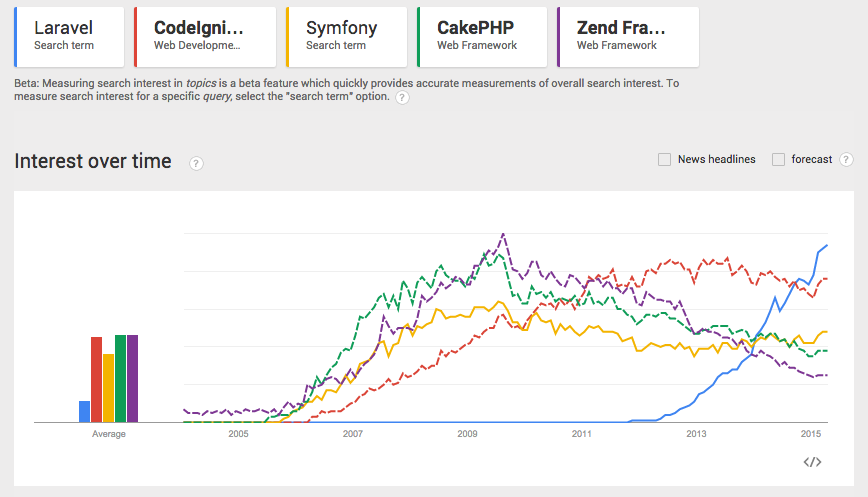
\includegraphics[width=1\textwidth]{images/trends-php-frameworks.png}
			\caption{Recherches Google pour les principaux frameworks PHP.}
			\label{fig:trends-php-frameworks}
		\end{figure}

		\subsubsection{Un framework MVC}
			Laravel est un framework mettant en avant une séparation très importante des modèles, des vues et des contrôleurs. Toutes les classes que nous avons créées se trouvent dans le dossier \verb|app| et sous l'espace de nom (\textit{namespace}) \verb|Diplo|.\\

			Nous avons choisi une architecture modulaire organisée selon les entités. À chaque entité on associe les fichiers suivants :
			\begin{itemize}
				\item \verb|Exceptions| : les exceptions de ce module ;
				\item \verb|Controllers| : les contrôleurs associés à l'entité ;
				\item \verb|Models| : les modèles associés à l'entité ;
				\item \verb|Repositories| : les classes d'accès aux bases de données ;
			\end{itemize}

		\subsubsection{Les \servicesProvider{}}
			Les \servicesProvider{} sont le centre de Laravel. Ce sont des classes qui permettent de lier des objets entre eux et d'enregistrer des éléments de configuration. Les \servicesProvider{} permettent d'enregistrer entre autres les éléments suivants:
			\begin{itemize}
				\item \textbf{La liaison entre les routes et les méthodes des contrôleurs}: ce qui permet qu'une méthode soit appelée en fonction de l'URL;
				\item \textbf{La liaison entre les événements et les listeners}: ce qui permet qu'une ou plusieurs classes listeners soient appelés lorsqu'un événement est levé;
				\item \textbf{La liaison entre les interfaces et les classes concrètes}: ce qui permet d'utiliser des interfaces partout dans l'application et de laisser Laravel injecter des classes concrètes plus tard.
			\end{itemize}\bigskip

			Les \servicesProvider{} se trouvent dans l'espace de nom \verb|Diplo\Providers|.

		\subsubsection{Injection de dépendance et \ioc{}}
		\label{subsubsec:ioc}
			Il est très rare d'instancier des classes lorsque l'on utilise Laravel. Tout d'abord, on peut remarquer que quand on enregistre des routes, on donne le nom du contrôleur, et non une instance de celui-ci. Laravel se charge de l'instanciation de la classe à notre place lorsque la route enregistrée est demandée. Pour instancier une classe, Laravel utilise un outil très puissant de résolution de dépendance se basant sur l'introspection de PHP. Avant de créer l'objet nécessaire, elle détermine les classes requises par le constructeur et les injecte. La résolution de dépendances est faite de manière récursive.\\

			En plus de la résolution automatique de dépendances, Laravel utilise l'\ioc{}. L'\ioc{} est un entrepôt de classes permettant de lier une interface à une implémentation concrète, où une chaîne de caractères à une classe par exemple. Cette dernière possibilité est présentée dans le listing \ref{code:ioc-container}.

			\begin{listing}[H]
				\inputminted[fontsize=\scriptsize]{php}{code/iocContainer.php}
				\caption{Un exemple d'utilisation de l'\ioc{}.}
				\label{code:ioc-container}
			\end{listing}

			Si le constructeur d'un contrôleur nécessite par exemple un objet \verb|Diplo\Messages\ConversationsRepository|, Laravel va utiliser l'injection de dépendance et l'\ioc{} afin de lui fournir une implémentation concrète qui aura été associée à l'interface. Cet exemple est présenté dans le listing \ref{code:ioc-controler}.
			\begin{listing}[H]
				\inputminted[fontsize=\scriptsize]{php}{code/injectionClass.php}
				\caption{Injection d'une interface dans un constructeur de contrôleur.}
				\label{code:ioc-controler}
			\end{listing}

			De cette manière, nous avons accès au répertoire dans notre contrôleur sans effort.

		\subsubsection{Les façades}
			Une façade est une classe spécifique qui permet d'appeler des méthodes publiques d'une instance d'un objet via des appels statiques sur la façade. Les classes qui peuvent être résolues par des façades sont celles qui se trouvent dans l'\ioc{} (abordé dans la partie \ref{subsubsec:ioc}).\\

			Par exemple, lorsque que l'on appelle une méthode statique sur la façade \verb|Route|, Laravel va en réalité appeler une méthode publique d'une instance d'une classe appelée \verb|Illuminate\Routing\Router| stockée dans l'application.\\

			On se retrouve alors avec deux possibilités dans les contrôleurs :
			\begin{itemize}
				\item utiliser des appels statiques via les façades ;
				\item injecter les véritables classes dans le constructeur et appeler des méthodes sur cette classe via un attribut de classe.
			\end{itemize}
			\vspace{10px}
			La deuxième option est généralement préférée, étant réputée \enquote{plus propre}. Pour autant l'utilisation des façades n'est pas totalement à proscrire.

		\subsubsection{Le \repositoryPattern}

			\paragraph{Description}
				Le \repositoryPattern{} est une bonne pratique de modélisation permettant d'abstraire la manipulation des données. Les objectifs sont nombreux :
				\begin{itemize}
					\item Uniformiser l’interaction avec les données à travers l'application ;
					\item Séparer la logique métier de l'accès aux données ;
					\item Faciliter les tests d'intégration en isolant la couche d'accès aux données ;
					\item Proposer plusieurs moyens d'accès aux données (bases de données, cache, fichiers, API\dots), tout en uniformisant les méthodes à l'aide d'interfaces.
				\end{itemize}

			\paragraph{Pourquoi utiliser des répertoires}
				Dans le cas d'une application plutôt simple comme la notre, il aurait été parfaitement correct d'appeler les méthodes de l'ORM\footnote{ORM : \textit{Object Relational Mapper.}} de Laravel, Eloquent, directement dans les contrôleurs.\\

				Mais dans le cas d'une application plus complexe, il est préférable de dissocier ses contrôleurs de l'ORM afin d'améliorer la maintenabilité de l'application et de permettre l'utilisation d'un autre système de stockage. En effet, si l'on décidait de passer à une autre méthode de stockage que celle choisie initialement, il faudrait aller chercher dans toute l'application où sont effectués ces accès. En utilisant le \repositoryPattern{} il suffit de créer une nouvelle classe respectant le contrat initial (l'interface créée) puis vérifier que celle-ci est conforme aux test écrits.

			\paragraph{Utilisation de répertoires}
				La création de répertoires est finalement assez simple. Les différentes étapes sont les suivantes:
				\begin{enumerate}
					\item Création d'une interface indiquant le comportement attendu pour l'accès aux données ;
					\item Création d'une classe concrète se conformant à l'interface en utilisant l'ORM de Laravel qui est Eloquent ;
					\item Association de l'interface à la classe concrète créée dans un \serviceProvider.
				\end{enumerate}

				Un exemple d'interface d'accès aux données concernant les parties est présenté dans le listing \ref{code:parties-repo-interface}. Son implémentation concrète est présentée dans le listing \ref{code:parties-repo-eloquent}.

				\begin{listing}[H]
					\inputminted[fontsize=\scriptsize]{php}{code/PartiesRepository.php}
					\caption{L'interface spécifiant le contrat d'accès aux données des parties.}
					\label{code:parties-repo-interface}
				\end{listing}

				\begin{code}
					\inputminted[fontsize=\scriptsize]{php}{code/EloquentPartiesRepository.php}
					\caption{Utilisation de l'ORM Eloquent pour l'accès aux données des parties.}
					\label{code:parties-repo-eloquent}
				\end{code}

	\subsection{Utilisation de \ppq{}}
		Nous avons fait le choix d'utiliser une architecture de type \ppq{} avec \url{http://www.iron.io} qui met à disposition des instances Iron en Push/Pull. Ce choix est justifié de la manière suivante:
		\begin{itemize}
			\item L'intégration d'Iron et des \ppq{} est immédiate dans Laravel;
			\item En utilisant une application SaaS\footnote{SaaS : \textit{Software As A Service}} nous n'avons pas besoin d'installer un nouveau service, de le configurer etc.;
			\item L'abonnement gratuit d'Iron.io nous laisse délivrer 1 million de messages par mois, ce qui nous apparaît comme suffisant vu l'ampleur de notre projet
		\end{itemize}\bigskip

		Nous utilisons des \ppq{} dans les cas suivants:
		\begin{itemize}
			\item \textbf{La création d'une carte quand une partie a assez de joueurs pour démarrer.} C'est une opération lente car il faut insérer les cases et les armées créées dans la base de données.
			\item \textbf{La fin d'une partie.} C'est une opération lente car il faut effectuer les actions relatives à la clôture de la partie.
			\item \textbf{Les changements de phases d'une partie.} C'est une opération qui doit être effectuée à un instant précis. Nous créons donc un message en queue, qui sera délivré à un instant précis et défini dans le futur. La réception de ce message ne ralentira pas les requêtes que peuvent faire les clients de l'API et s'occupera du changement d'état de la partie.
		\end{itemize}
\section{Côté client}
